% !TeX encoding = UTF-8
% !TeX spellcheck = sk_SK
% !TeX root=tukedip.tex

\section{Implementácia projektu}
V tejto časti podrobne opíšeme realizáciu nášho projektu. Opíšeme architektúru systému a účel jednotlivých modulov. Poskytneme aj prehľad štruktúry kódu a funkčnosti jednotlivých súborov. Okrem toho vysvetlíme, ako sme do nášho projektu integrovali rôzne technológie a knižnice, aby sme dosiahli naše ciele. Nakoniec rozoberieme všetky problémy, s ktorými sme sa stretli počas procesu implementácie, a ako sme ich riešili.
\subsection{Prehľad štruktúry programov} 

    \begin{center}
        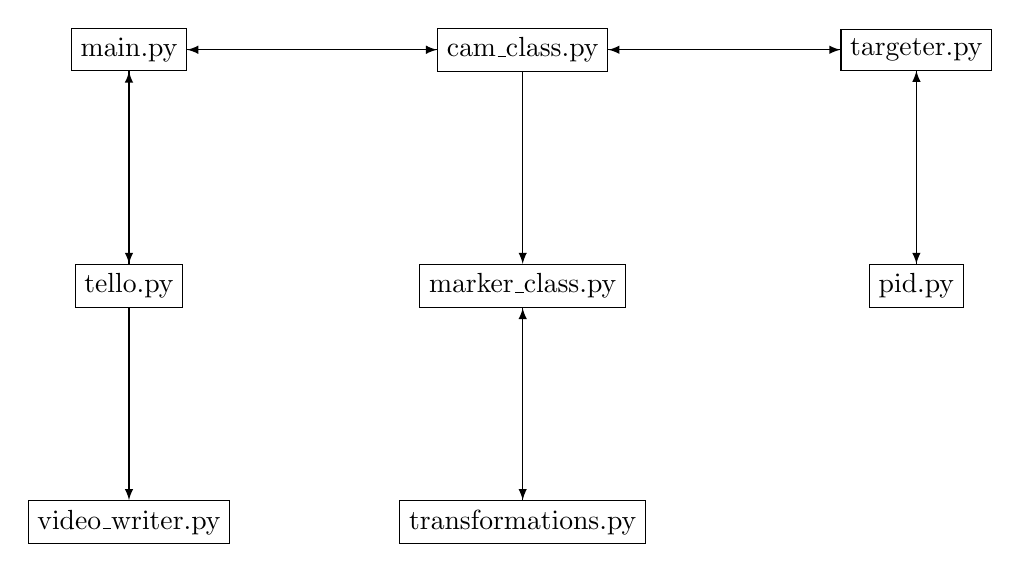
\begin{tikzpicture}[node distance=3cm]
            \node (main) [draw, rectangle] {main.py};
            \node (tello) [draw, rectangle, below of=main] {tello.py};
            \node (cam) [draw, rectangle, right of=main, xshift=2cm] {cam\_class.py};
            \node (targeter) [draw, rectangle, right of=cam, xshift=2cm] {targeter.py};
            \node (video) [draw, rectangle, below of=tello] {video\_writer.py};
            \node (marker) [draw, rectangle, below of=cam] {marker\_class.py};
            \node (pid) [draw, rectangle, below of=targeter] {pid.py};
            \node (transform) [draw, rectangle, below of=marker] {transformations.py};

            \draw[-latex] (main) -- (tello);
            \draw[-latex] (tello) -- (main);
            \draw[-latex] (main) -- (cam);
            \draw[-latex] (cam) -- (main);
            \draw[-latex] (cam) -- (targeter);
            \draw[-latex] (targeter) -- (cam);
            \draw[-latex] (targeter) -- (pid);
            \draw[-latex] (pid) -- (targeter);
            \draw[-latex] (tello) -- (video);
            \draw[-latex] (cam) -- (marker);
            \draw[-latex] (marker) -- (transform);
            \draw[-latex] (transform) -- (marker);
        \end{tikzpicture}
    \end{center}

    \textbf{Popis:}

    \textbf{main.py} - Obsahuje grafické rozhranie pyGame a zobrazenie obrazu kamery. Používa rôzne klávesy na klávesnici na prepínanie funkcií alebo ovládanie dronu.

    \textbf{tello.py} - Obsahuje funkcie na komunikáciu s dronom a čítanie údajov.

    \textbf{video\_writer.py} - Beží na samostatnom vlákne, zachytáva video počas automatického ovládania a potom ho vypúšťa.

    \textbf{cam\_class.py} - Vykonáva úlohy spracovania obrazu (kalibrácia, rozpoznávanie značiek) a údaje o rýchlosti dronu sa odtiaľto zaraďujú do frontu. Odovzdáva načítané pozície značiek funkciám, ktoré ich spracúvajú.

    \textbf{targeter.py} - Prečíta funkcie zodpovedajúce poradovým číslam značiek zo zadaného súboru CSV a vráti vektor kontrolnej základne.

    \textbf{pid.py} - Obsahuje triedu implementujúcu numerický PID regulátor, vypočítava hodnoty regulačného stupňa.

    \textbf{marker\_class.py} - Trieda, ktorá uchováva všetky údaje pre značky. Počas zberu údajov počíta a nakoniec zapisuje zozbierané pozície do súboru NPZ.
 
    \textbf{transformations.py} - Implementuje transformácie súradnicového systému a obsahuje funkcie na konverziu vektorov rotácie.

 
\subsection{Ovládanie drona}
Dron Tello sa ovláda pomocou kombinácie softvérových programov, ktoré s ním komunikujú prostredníctvom pripojenia Wi-Fi (obrázok 4-1). Na nízkoúrovňovú komunikáciu medzi dronom a riadiacim počítačom sa používa knižnica Tello Python, tello.py.

\begin{figure}[ht!]
    \centering
    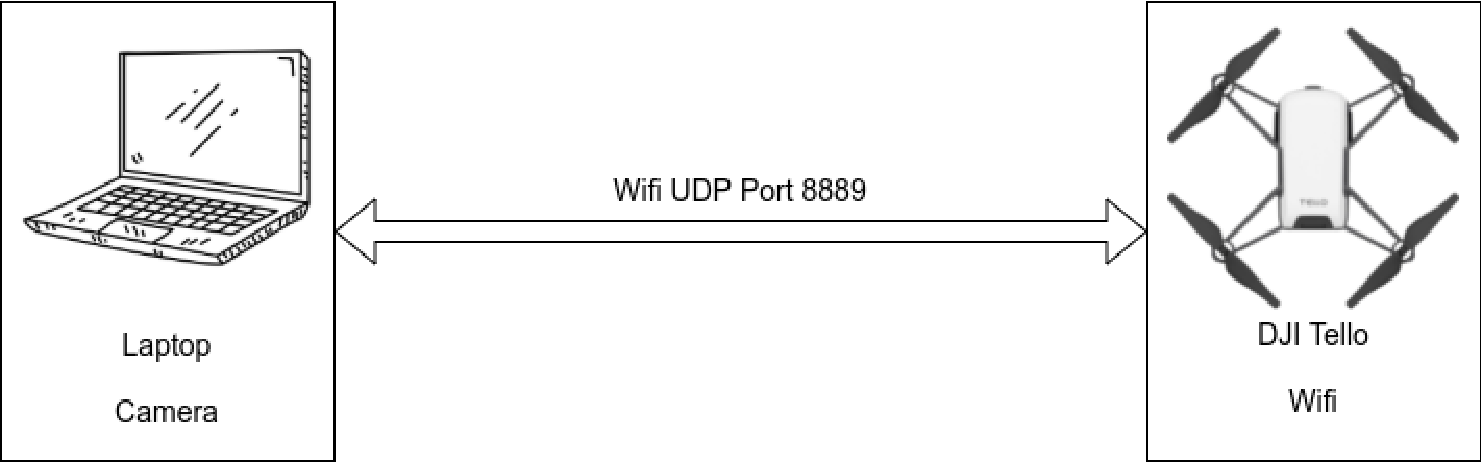
\includegraphics[width=.70\textwidth,angle=0]{figure 4-3.pdf}
    \caption{Schéma procesu pripojenia dronu.}
    \captionsetup{font=footnotesize, justification=centering, skip=5pt}
    \caption*{(Zdroj: vlastné spracovanie)}
    \label{o:4-3} 
\end{figure}  

Knižnica tello.py poskytuje množstvo funkcií, ktoré možno použiť na odosielanie príkazov do dronu a prijímanie údajov z neho. Medzi tieto funkcie patria 
$takeoff()$, $land()$, $move\_left()$, $move\_right()$, $move\_forward()$, $move\_backward()$, \break $rotate\_clockwise()$, $rotate\_counter\_clockwise()$ 
a mnohé ďalšie. Knižnica obsahuje aj funkcie na získavanie údajov z dronu, ako je jeho aktuálna výška, úroveň nabitia batérie a čas letu.

Na ovládanie dronu Tello z webovej aplikácie program využíva spojenie "web-sockets" na komunikáciu so skriptom Python na strane servera. Tento skript funguje ako most medzi webovou aplikáciou a dronom Tello a prenáša medzi nimi príkazy a údaje.

Skript na strane servera používa knižnicu tello.py na odosielanie príkazov do dronu a prijímanie údajov z neho. Keď používateľ zadá príkaz vo webovej aplikácii, príkaz sa odošle na server prostredníctvom spojenia "web-sockets". Server potom použije príslušnú funkciu v knižnici tello.py na odoslanie príkazu dronu. Po vykonaní príkazu môže server získať všetky relevantné údaje z dronu a poslať ich späť do webovej aplikácie na zobrazenie.

Celkovo kombinácia tello.py a skriptu na strane servera poskytuje výkonnú platformu na ovládanie dronu Tello z webovej aplikácie. Vďaka možnosti odosielať širokú škálu príkazov a získavať podrobné údaje z dronu.

\subsection{Spracovanie obrázkov}
S riadením dronov úzko súvisí, ale viac sa zaoberá spracovaním obrazu, program cam\_class.py, ktorého hlavná funkcia je zodpovedná za rozpoznávanie značiek ArUco. ArUco značky sa zisťujú pomocou vstavanej funkcie OpenCV cv2.aruco.detectMarkers(). Tá nájde kódy v načítanom zväzku značiek po adaptívnej segmentácii aplikovanej na obraz v odtieňoch sivej a vráti ich rohové body v pixeloch a ich poradové číslo. Na výpočet skutočnej trojrozmernej polohy značiek na základe matíc kamery sa používa už spomínaná transformácia PnP. Výsledné polohy s ich poradovým číslom značky sa môžu odoslať na ďalšie spracovanie (časť 4.4) alebo použiť na automatickú navigáciu dronu.

Program je určený na navigáciu dronu Tello pomocou značiek umiestnených na zemi. To sa dosiahne použitím knižnice OpenCV na detekciu značiek vo videozázname z kamery dronu.
\begin{mypython}[caption={Inicializácia parametrov detekcie značiek OpenCV},label=CL-3]

    import cv2
    import numpy as np
    from djitellopy import Tello
    
    # Initialize Tello drone
    tello = Tello()
    tello.connect()
    tello.streamon()
    
    # Initialize OpenCV marker detection parameters
    aruco_dict = cv2.aruco.Dictionary_get(cv2.aruco.DICT_6X6_250)
    aruco_params = cv2.aruco.DetectorParameters_create()
    
    # Set up video stream
    stream = tello.get_video_stream()
\end{mypython}

Program najprv inicializuje kameru a nastaví tok videa. Potom pomocou slučky nepretržite zachytáva snímky z videoprenosu a spracováva ich. Pre každú snímku program používa vstavané funkcie OpenCV na detekciu značiek a odhad ich polohy v 3D priestore.
\begin{mypython}[caption={Detekcia značky a vypočítanie polohy},label=CL-4]
    while True:
    # Capture frame from video stream
    frame = stream.read()

    # Detect markers in frame
    corners, ids, rejected = cv2.aruco.detectMarkers(frame, aruco_dict, parameters=aruco_params)

    # Estimate marker position in 3D space
    rvecs, tvecs, _ = cv2.aruco.estimatePoseSingleMarkers(corners, 0.05, camera_matrix, dist_coeffs)

    # Process marker positions
    if ids is not None:
        # TODO: Implement control algorithm
        pass

    # Display frame
    cv2.imshow('Frame', frame)
    if cv2.waitKey(1) & 0xFF == ord('q'):
        break

\end{mypython}

Po odhadnutí polohy značiek program pomocou proporcionálneho riadiaceho algoritmu upravuje odklon, sklon a výšku dronu na základe polohy značiek vzhľadom na stred snímky. Algoritmus vypočíta chybu medzi stredom rámu a polohou značiek a upraví orientáciu a výšku dronu tak, aby sa táto chyba minimalizovala.

Program obsahuje aj niekoľko bezpečnostných funkcií, ktoré zabraňujú kolízii dronu s prekážkami alebo vyleteniu mimo dosahu. Medzi tieto funkcie patrí nastavenie maximálnej výšky a doletu dronu, ako aj detekcia prekážok v dráhe dronu a automatické nastavenie jeho trajektórie tak, aby sa im vyhol.

Na ďalšie zlepšenie presnosti a spoľahlivosti detekcie a sledovania značiek program obsahuje množstvo konfigurovateľných parametrov, ako je minimálna a maximálna veľkosť značky, prah detekcie a proporcionálne zisky riadenia. Tieto parametre sa dajú upraviť tak, aby sa optimalizoval výkon programu pre rôzne prostredia a svetelné podmienky.

Celkovo program poskytuje spoľahlivý a efektívny spôsob navigácie dronu Tello pomocou značkovačov. Použitím knižnice OpenCV na detekciu a sledovanie značiek v reálnom čase a implementáciou proporcionálneho riadiaceho algoritmu na úpravu orientácie a výšky dronu je program schopný navigovať dron s vysokou mierou presnosti a precíznosti.

\subsection{Spracovanie údajov}
Spracovanie priestorových bodov a rotácií získaných z programov na spracovanie obrazu z kamery, t. j. zber údajov, vykonáva program marker\_class.py. Potrebné transformácie, ktoré sú opísané vyššie, vykonávajú funkcie transformations.py.
\subsubsection{Ukladanie údajov o značkách}
Na spracovanie sa môžu odovzdať len údaje značiek, ktoré nemajú žiadny zo svojich vrcholov v pixelovom rámci obrazu. Definícia hrany je 2-2-2-2 \% priesečník na všetkých štyroch stranách obrazu kamery. Značkovače umiestnené na okrajoch poskytujú po odstránení skreslenia jednak nepresnejšie údaje, jednak môžu spôsobiť neistotu označenia vonkajších okrajov 2D kódu značkovača počas detekcie značkovača, ako je to vidieť na obrázku 20.
%TODO: obrazok

V triede markers sú vlastnosti značiek, ktoré ste doteraz videli, uložené v rôznych zoznamoch, ako napríklad:
\begin{itemize}
    \item \textbf{ids}: počet už použitých značiek
    \item \textbf{tvec\_origin}: "markerorigos" v globálnom súradnicovom systéme
    \item \textbf{rvec\_origin}: otočenie súradnicového systému značiek vzhľadom na globálny
    \item \textbf{dRot}: matica rotácie od danéj značky ku globálnemu.
    \item \textbf{allow\_use}: pomocná premenná, ktorá umožňuje použitie danéj značky pri priemerovaní, akonáhle sa zozbiera dostatočný počet vzoriek, môže sa započítať
    \item \textbf{tvec\_min, tvec\_max}: pomocné premenné na filtrovanie výpočtu priemeru
\end{itemize}

Funkcia appendMarker() volaná počas detekcie značiek ArUco pridá nové značky do triedy značiek. Za počiatok berie značku s číslom 1 a na základe jej Eulerovho uhlového natočenia okolo osi x určí, či ide o horizontálnu alebo vertikálnu značku. Ukladá tiež základné hodnoty uhlových rotácií z čítania stavov dronu, to sa stáva počiatkom Eulerových uhlov. Ukladá príslušnú jednu z dvoch orientácií do matice, ktorá bude relevantná pre indexovanie po spracovaní invertovaním smerov vektora translácie.

Ďalšie značky sa ukladajú vytvorením transformácií medzi súradnicovými systémami, ktoré sú implementované skriptom getTransformations() v súbore transformations.py. V prevádzke systém v súčasnosti pracuje s 12 platnými vzormi. Testy boli vykonané s vyššími limitmi platnosti, ale mnohokrát systém nestihol vykonať transformácie, kým sa značky nenachádzali v zornom poli dronu a nebol schopný vypočítať ďalšie. Preto sa zozbiera 12 vektorov posunu medzi dvoma značkami, pričom sa vyradia minimálne a maximálne normály a z 10 zostávajúcich hodnôt sa vytvorí priemer. Matice natočenia sa tiež získajú spriemerovaním 12 vzoriek bez filtrovania. Výsledné hodnoty sa uložia do zoznamov objektov triedy.

Ak už má značka vzorku na autorizáciu, možno ju spočítať pomocou funkcie v úryvku kódu 5. Program spočíta pozície načítané zo všetkých pozorovaných značiek, spriemeruje ich a uloží túto hodnotu pozície. Od uhlových natočení načítaných zo snímača dronu odpočíta počiatok uhlov, čím získa orientáciu dronu.
    % """
    % Calculates the position of the camera relative to the marker, given the marker position and orientation,
    % and the camera position and orientation.
    % Arguments:
    % - marker_pos: A numpy array representing the position of the marker in 3D space.
    % - marker_orient: A numpy array representing the orientation of the marker in 3D space.
    % - camera_pos: A numpy array representing the position of the camera in 3D space.
    % - camera_orient: A numpy array representing the orientation of the camera in 3D space.
    % Returns:
    % - A numpy array representing the position of the camera relative to the marker in 3D space.
    % """
\begin{mypython}[caption={Vypočíta polohu kamery vzhľadom na značku},label=CL-4]
    def calculate_position(marker_pos, marker_orient, camera_pos, camera_orient):
    # rotation matrix for the marker orientation
    marker_rot = cv2.Rodrigues(marker_orient)[0]
    # rotation matrix for the camera orientation
    camera_rot = cv2.Rodrigues(camera_orient)[0]
    # transformation matrix from marker to camera coordinates
    marker_to_camera = np.hstack((marker_rot.T, -marker_rot.T.dot(marker_pos.reshape(3,1))))
    # transformation matrix from camera to global coordinates
    camera_to_global = np.hstack((camera_rot, camera_pos.reshape(3,1)))
    # transformation matrix from marker to global coordinates
    marker_to_global = camera_to_global.dot(marker_to_camera)
    # position of the camera relative to the marker
    camera_rel_marker = marker_to_global[:,3]
    
    return camera_rel_marker
\end{mypython}
\subsection{Webová aplikácia}
Vývoj webovej aplikácie je základnou súčasťou riadiaceho systému pre viacero dronov Tello. Táto webová aplikácia slúži ako používateľské rozhranie na ovládanie dronov v individuálnom aj skupinovom režime. S cieľom zabezpečiť bezproblémové a používateľsky prívetivé prostredie je webová aplikácia navrhnutá s moderným a intuitívnym rozhraním s využitím najnovších technológií vývoja webových aplikácií.

Webová aplikácia je rozdelená na dve hlavné zložky: frontend a backend(obrázok 4-2). Frontend je zodpovedný za prezentáciu používateľského rozhrania a obsluhu interakcie používateľa, zatiaľ čo backend zabezpečuje komunikáciu medzi webovou aplikáciou a dronmi.

\begin{figure}[ht!]
    \centering
    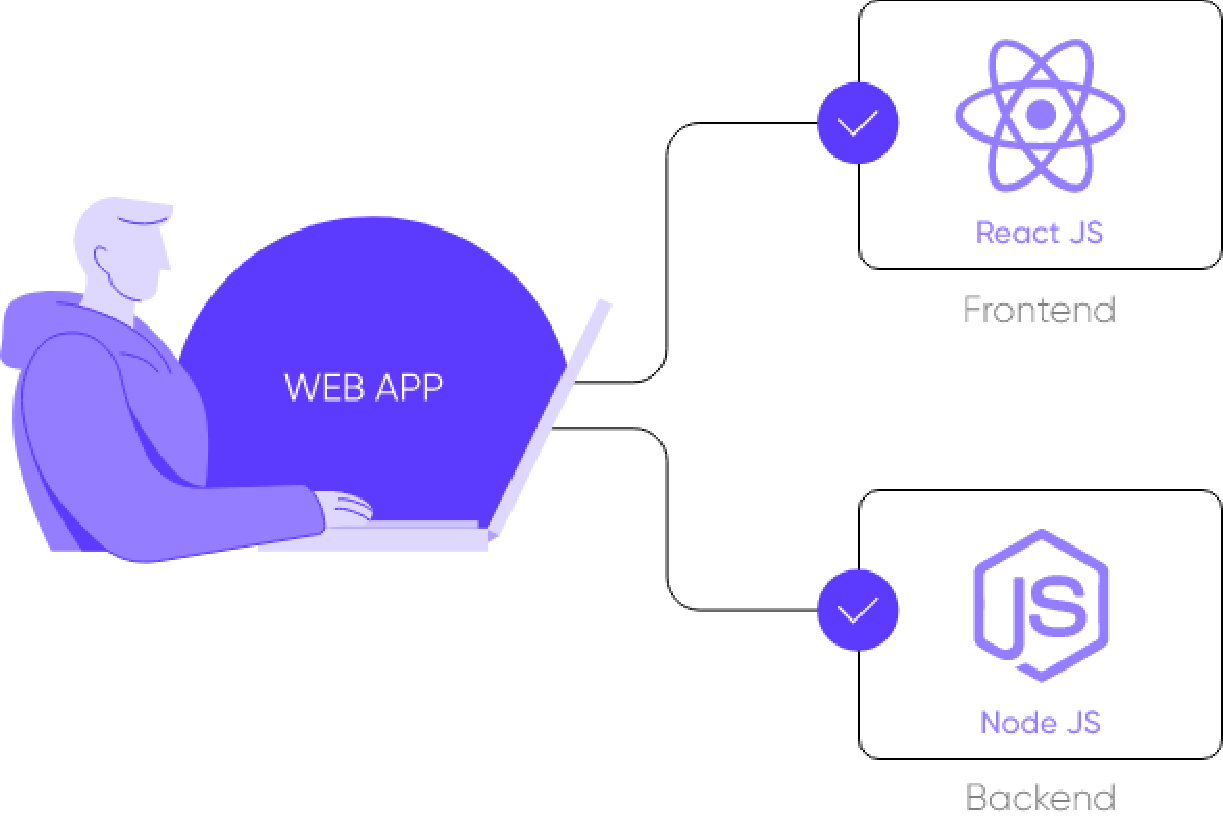
\includegraphics[width=.50\textwidth,angle=0]{figure 4-2.pdf}
    \caption{Schéma rozdelenia webovej aplikácie.}
    \captionsetup{font=footnotesize, justification=centering, skip=5pt}
    \caption*{(Zdroj: vlastné spracovanie)}
    \label{o:4-2}
\end{figure}  

\subsubsection{Frontend}
Webová aplikácia React sa skladá z viacerých komponentov, ktoré spolupracujú pri ovládaní dronov. Keď sa používateľ prihlási do aplikácie, zobrazí sa mu ovládací panel, na ktorom sú zobrazené dostupné drony a ich stav. Informačný panel sa aktualizuje v reálnom čase pomocou webových soketov, aby odrážal zmeny stavu dronov.

Komponent ovládania dronov umožňuje používateľovi vybrať dron a ovládať jeho pohyb pomocou virtuálneho joysticku. Komponent joystick je vytvorený pomocou vlastného rozhrania joysticku. Keď používateľ pohybuje joystickom, komponent posiela príkazy do letového ovládača dronu prostredníctvom webových soketov. Pohyb dronu sa aktualizuje v reálnom čase.

Komponent telemetrie dronu poskytuje v reálnom čase spätnú väzbu o stave dronu vrátane jeho výšky, úrovne nabitia batérie a polohy GPS. Komponent prijíma telemetrické údaje z letového ovládača dronu prostredníctvom pripojenia WebSocket a aktualizuje prístrojový panel s najnovšími informáciami.

Funkčný komponent React, ktorý slúži ako hlavný vstupný bod aplikácie, používa háčik useState na správu stavu rôznych premenných, ktoré určujú aktuálny stav dronu, napríklad jeho nadmorskú výšku, rýchlosť a úroveň batérie. Háčik useEffect sa používa na vykonávanie vedľajších efektov, ako je prihlásenie sa k udalostiam zo servera WebSocket, aktualizácia používateľského rozhrania v reakcii na zmeny stavu a vyčistenie zdrojov, keď je komponent odpojený.

Háčik useContext sa používa na zdieľanie stavu a funkcií medzi rôznymi komponentmi aplikácie. To umožňuje vytvoriť modulárnejšiu a udržiavateľnejšiu kódovú základňu, pretože každá zložka musí vedieť len o stave a funkciách, ktoré sú relevantné pre jej funkčnosť.

Komponenty Material UI, ktoré sa v aplikácii používajú, poskytujú konzistentné a vizuálne príťažlivé používateľské rozhranie. Mriežka sa používa na responzívne a flexibilné rozloženie rôznych komponentov, zatiaľ čo ToggleButton, Tabs, Tab, Button, Typography a Box sa používajú na poskytovanie tlačidiel, štítkov a iných prvkov používateľského rozhrania.

Vlastná komponenta BatteryGauge sa používa na zobrazenie aktuálnej úrovne nabitia batérie dronu vizuálne príťažlivým a zrozumiteľným spôsobom. Komponent ControlBlock vykresľuje niekoľko komponentov NavigationButton, ktoré umožňujú používateľovi ovládať pohyb dronu a ďalšie funkcie.

Nakoniec sa aplikácia pripája k serveru WebSocket pomocou knižnice socket.io-client. To umožňuje komunikáciu medzi aplikáciou a dronom v reálnom čase, vďaka čomu môže používateľ ovládať pohyb dronu a prijímať aktualizácie o jeho stave. Aplikácia počúva rôzne udalosti zo servera, ako napríklad "zmena výšky" a "zmena stavu batérie", a podľa toho aktualizuje stav príslušných premenných. Celá táto infraštruktúra je znázornená na obrázku 4-3.

\begin{figure}[ht!]
    \centering
    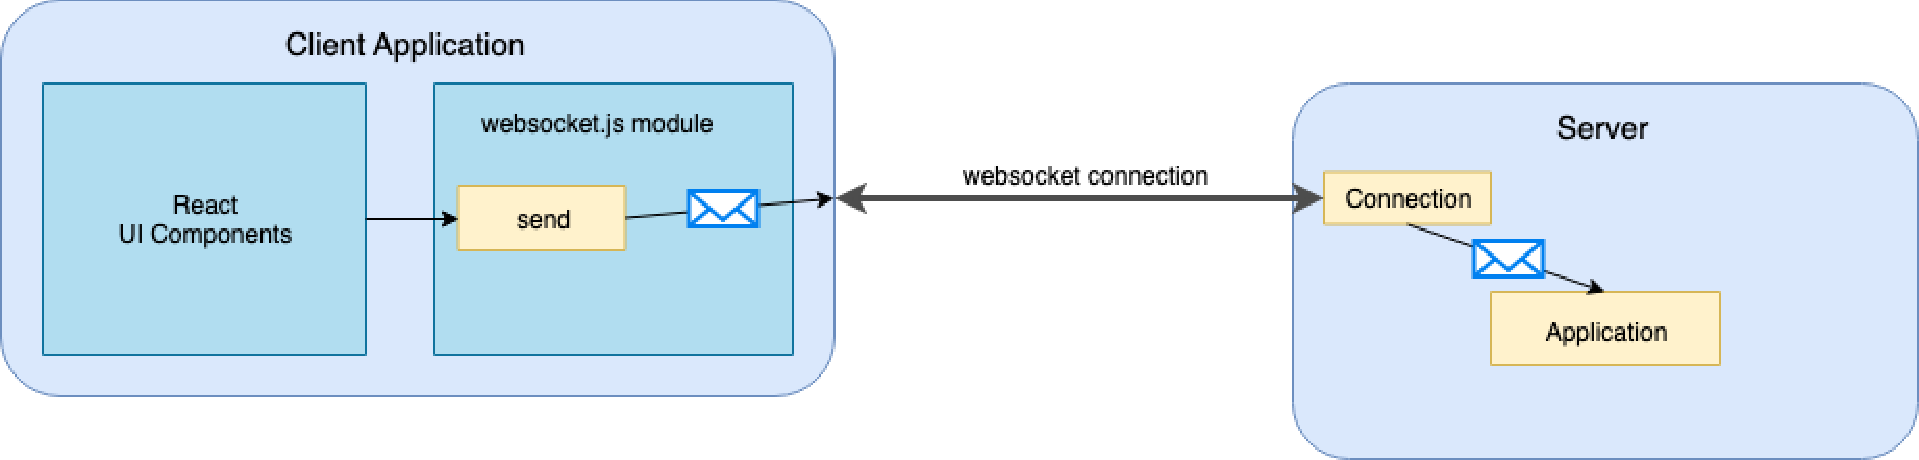
\includegraphics[width=.99\textwidth,angle=0]{figure 4-1.pdf}
    \caption{Schéma webovej aplikácie.}
    \captionsetup{font=footnotesize, justification=centering, skip=5pt}
    \caption*{(Zdroj: vlastné spracovanie)}
    \label{o:4-1}
\end{figure}  

\subsubsection{Backend}
Server Node.js poskytuje backendové funkcie pre webovú aplikáciu na ovládanie dronov. Server je vytvorený pomocou frameworku Express.js a používa knižnicu Socket.IO na vytvorenie spojenia v reálnom čase medzi webovou aplikáciou a dronmi.

Server počúva spojenia pomocou metódy io.on(), ktorá sa zavolá vždy, keď sa klient pripojí k serveru. Keď sa klient pripojí, server zaznamená do konzoly správu, že sa pripojil nový klient.

Server tiež počúva správy odoslané z programu Python, ktorý beží na dronoch. Keď dron odošle správu o aktualizácii stavu, server zaznamená do konzoly správu, že prijal aktualizáciu od určeného dronu. Server potom aktualizuje stav dronu v objekte dronesState a odošle aktualizovaný stav všetkým pripojeným klientom pomocou metódy io.sockets.emit().

Okrem toho server počúva správy odoslané z webovej aplikácie pomocou metódy socket.on(). Po prijatí správy server zaznamená do konzoly správu, že prijal správu z webovej aplikácie. Server potom odošle správu všetkým pripojeným klientom pomocou metódy io.sockets.emit().

Server sa spustí na zadanom porte pomocou metódy server.listen(). Ak nie je zadaný žiadny port, server sa predvolene nastaví na port 3000. Po spustení servera sa do konzoly zaznamená správa, že server počúva na zadanom porte.

Celkovo server Node.js zohráva kľúčovú úlohu pri uľahčovaní komunikácie v reálnom čase medzi webovou aplikáciou a dronmi, čo umožňuje presné riadenie a monitorovanie pohybu a stavu dronov.